% Licensed to the Apache Software Foundation (ASF) under one or more
% contributor license agreements. See the NOTICE file distributed with
% this work for additional information regarding copyright ownership.
% The ASF licenses this file to You under the Apache License, Version 2.0
% (the ``License''); you may not use this file except in compliance with
% the License. You may obtain a copy of the License at
%
% http://www.apache.org/licenses/LICENSE-2.0
%
% Unless required by applicable law or agreed to in writing, software
% distributed under the License is distributed on an ``AS IS'' BASIS,
% WITHOUT WARRANTIES OR CONDITIONS OF ANY KIND, either express or implied.
% See the License for the specific language governing permissions and
% limitations under the License.

\subsubsection{Configuring an RSS Connector}

You must fill in the following tabs if you are configuring an RSS
Connector:

\bigimage{RSS-edit-repository-tab3}

\begin{itemize}

\item \textbf{Max connections (per JVM):} Here you can set the maximum
number of connections to your repository.  \ifCombinedConnectorGuide
The maximum number of connections per JVM is important for three
reasons; licensing, appliance resources, and the possiblity of
overwhelming the ingestion interface. For a more complete explanation,
see the Max Connections item on page \pageref{maxrepocon}.\fi

\ifJDBCGuide
The maximum number of connections per JVM is important for two reasons.
First, the number of connections may impact the resources
available on the appliance. If the connector framework is slowing down
your appliance, lowering this number should help.

Second, only ten document streams can be processed by the appliance
at one time.  If you are also using other repository connectors or
the \command{ingest} command on the appliance, you should reduce this
number to prevent contention for the Ingestion interface. The RSS
Connector will never overwhelm the interface on its own, but when other
applications are also using the ingestion interface, it may be best to
set the number of repository connections to five or even fewer.
\fi


\item \textbf{Throttling:} Here you can set a maximum average document fetch
rate for the repository connection. The maximum fetch rate allows you
to set three things: Expression, description, and fetches per minute.

In the RSS Connector, the value set in the expression field is a
server name. To throttle an individual server, use its name as the
expression and set the number of document fetches per minute. We
recommend a maximum average rate of 6 fetches per minute.  Once you
have set that, click Add.
\end{itemize}

In general, you should be conscientious about document fetch rates,
feed query rates, download rates, and other rates related to server
traffic when using the RSS Connector to connect to public, external
servers. The recommended rates suggested in this guide are typically
an upper limit. You should not exceed these suggestions for external
servers. Higher demands on these servers may produce undesirable
effects in their performance; the administrators of those servers may
block your connection.

If your organization uses RSS publishing internally, you should speak
to your server administrators about appropriate rate limits.

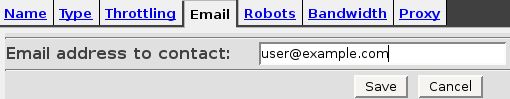
\includegraphics[width=300pt]{RSS-edit-repository-tab4}

\begin{itemize}

\item \textbf{Email:} A contact email address. This email address is included in request headers sent to servers. Administrators of servers recieving these requests may wish to contact you regarding your interactions with their content servers.

\end{itemize}

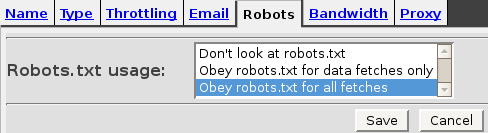
\includegraphics[width=300pt]{RSS-edit-repository-tab5}

\begin{itemize}

\item \textbf{Robots.txt Usage:} This determines whether the crawler obeys guidelines from the \dirpath{robots.txt} file on a server. There are three options:

\begin{itemize}

\item \textbf{Don't look at robots.txt}

\item \textbf{Obey robots.txt for data fetches only}

\item \textbf{Obey robots.txt for all fetches}

\end{itemize}

By default, \textbf{Obey robots.txt for all fetches} is selected. When
selected, the crawler will obey all interfacing and downloading
guidelines set in a server's \dirpath{robots.txt} file. You should
always use this setting when connecting to servers on the open Internet.

\end{itemize}

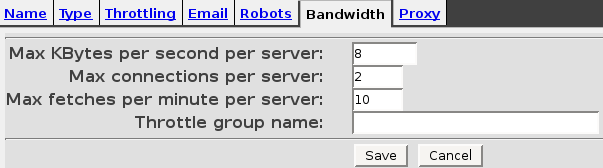
\includegraphics[width=300pt]{RSS-edit-repository-tab6}

\begin{itemize}


\item \textbf{Max KBytes per second per server:} The maximum download rate
from each server, which will include all content from that server. This
should be no more than 8 kilobytes per second for servers on the open
Internet

\item \textbf{Max connections per server:} The maximum number of
connections to each server. This should be 1 or 2 for servers on the
open Internet.

\item \textbf{Max fetches per minute per server:} The maximum number of
document fetches per minute for each server. This should be no higher
than 10 fetches per minute for servers on the open Internet.

\item \textbf{Throttle group name:} (Optional) Connections that have the
same throttle group name will be throttled together. A blank name will
match all other named groups. You should give repository connections
that will be used to crawl the same servers the same throttle group name.

\end{itemize}

If your organization uses RSS publishing internally, you should
consult your system administrator about appropriate limits.

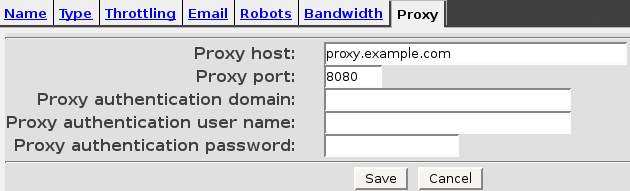
\includegraphics[width=300pt]{RSS-edit-repository-tab7}

This tab allows you to set up a proxy host if your MetaCarta appliance
needs a proxy server to forward requests outside of your
local network. If your appliance and proxy server are part of an NTLM
domain, you will need to include domain information and a user name
and password associated with that domain that has access to the proxy
server.

\begin{itemize}

\item \textbf{Proxy host:} The proxy server host name.

\item \textbf{Proxy port:} The port used to communicate with the proxy server. Often, this is port 8080. Ask the administrator of your proxy server for the port number you should enter here.

\item \textbf{Proxy authentication domain:} (Optional) The NTLM authentication domain of the proxy server and appliance.

\item \textbf{Proxy authentication user name:} (Optional) The user name given to the appliance for use in the domain. This user name should have access to the proxy server.

\item \textbf{Proxy authentication password:} (Optional) The password corresponding with that user name.

\end{itemize}


After entering this information, you will be taken to the repository
connection status page for this repository:

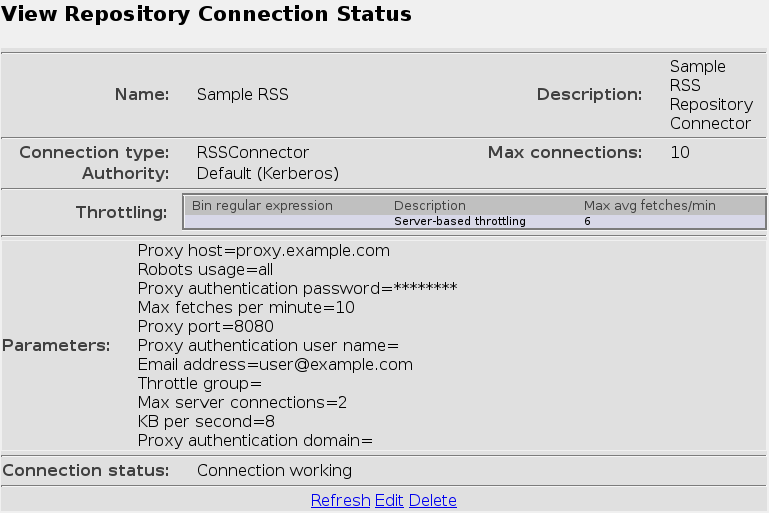
\includegraphics[width=300pt]{RSS-view-repo-conn-status}

In this example, the Connection Status is ``Connection working.''  If the
Connection Status is ``Connection failed,'' you might have have entered
some information (particularly your proxy information) incorrectly. If
so, click ``Edit'' to fix the data.
